\chapter{Results}
\label{cha:result}




\section{Pacman}\
\label{sec:pacman}
\subsection{Agent Performance} 


\begin{figure*}[!hbtp]
  \label{fig:cost}
  \makebox[\textwidth]{\framebox[5cm]{\rule{0pt}{5cm}}}
\caption{This is a placeholder.{\label{pacman_performance}}}
  
 % \subfigure[Fraction of cycles spent on zeroing\label{fig:zerocost}]{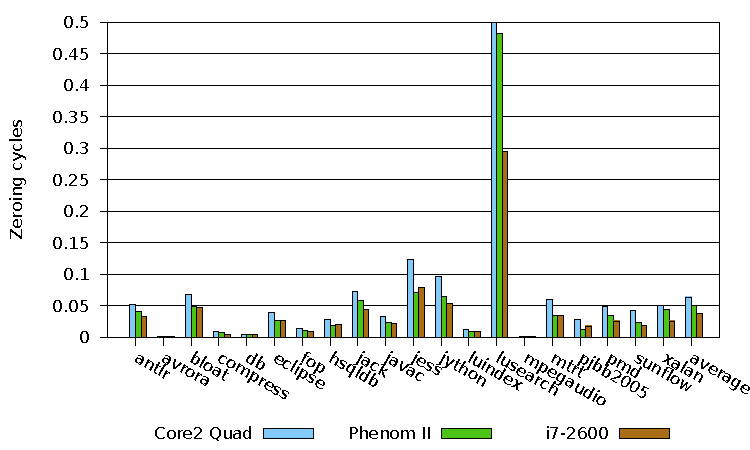
\includegraphics[width=\columnwidth]{figs/zerocost_intel.pdf}}
%  \subfigure[BytesZeroed / BytesBurstTransactionsTransferred\label{fig:zerobus}]{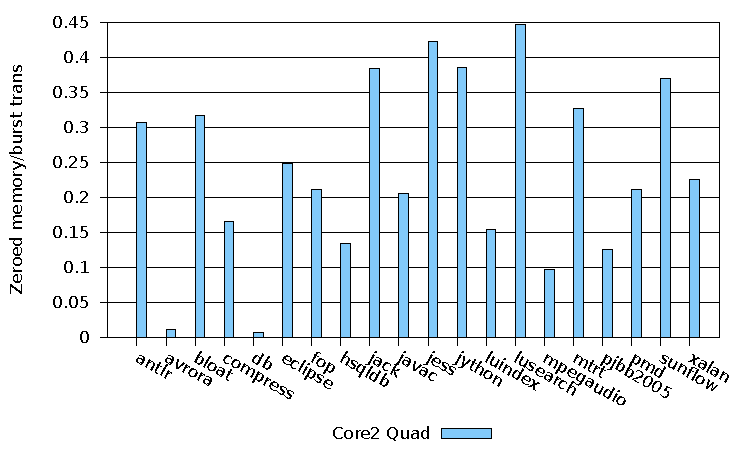
\includegraphics[width=1.0\columnwidth]{figs/zerobus_core.pdf}}



\end{figure*}


\subsection{Analysis}
%%%%%%%%%%%%
%%%%%%%%%%%%


\section{Tic-Tac-Toe}\
\label{sec:tic_tac_toe}
\subsection{Agent Performance} 


\begin{figure*}[!hbtp]
  \label{fig:cost}
  \makebox[\textwidth]{\framebox[5cm]{\rule{0pt}{5cm}}}
\caption{This is a placeholder.{\label{tic_tac_toe_performance}}}
  
 % \subfigure[Fraction of cycles spent on zeroing\label{fig:zerocost}]{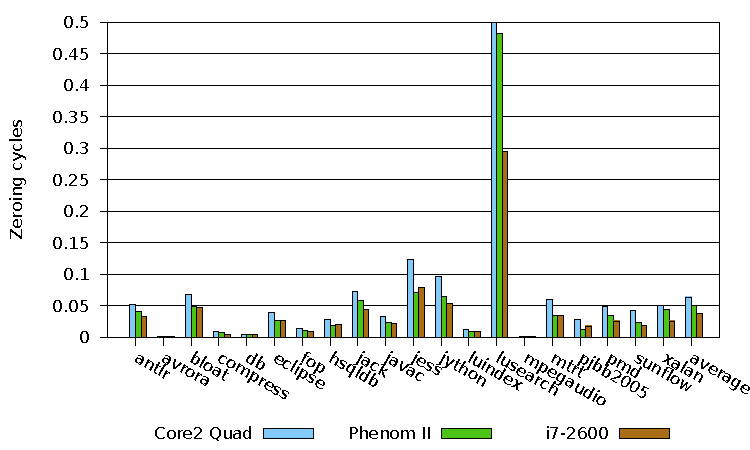
\includegraphics[width=\columnwidth]{figs/zerocost_intel.pdf}}
%  \subfigure[BytesZeroed / BytesBurstTransactionsTransferred\label{fig:zerobus}]{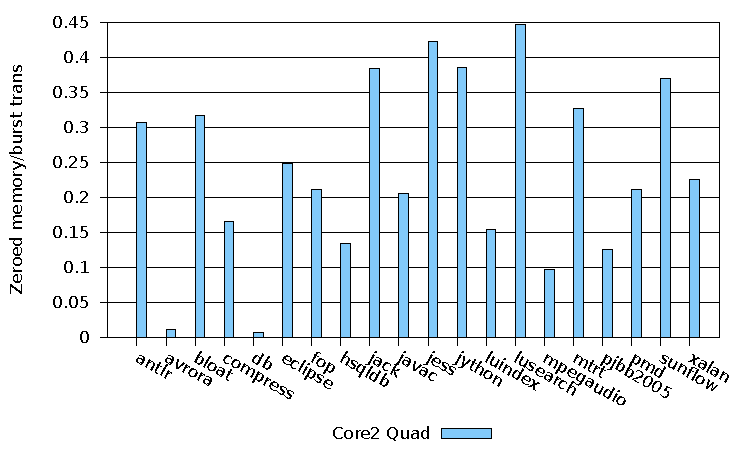
\includegraphics[width=1.0\columnwidth]{figs/zerobus_core.pdf}}



\end{figure*}



\subsection{Analysis}



%%%%%%%%%%%%
%%%%%%%%%%%%

\section{Biased Rock-Paper-Scissor}\
\label{sec:biased_rock_paper_scissor}
\subsection{Agent Performance} 

\begin{figure*}[!hbtp]
  \label{fig:cost}
  \makebox[\textwidth]{\framebox[5cm]{\rule{0pt}{5cm}}}
\caption{This is a placeholder.{\label{biased_rock_paper_scissor_performance}}}
  
 % \subfigure[Fraction of cycles spent on zeroing\label{fig:zerocost}]{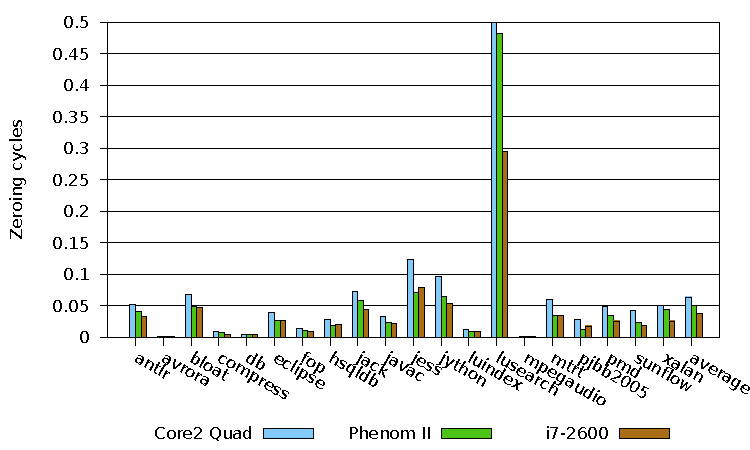
\includegraphics[width=\columnwidth]{figs/zerocost_intel.pdf}}
%  \subfigure[BytesZeroed / BytesBurstTransactionsTransferred\label{fig:zerobus}]{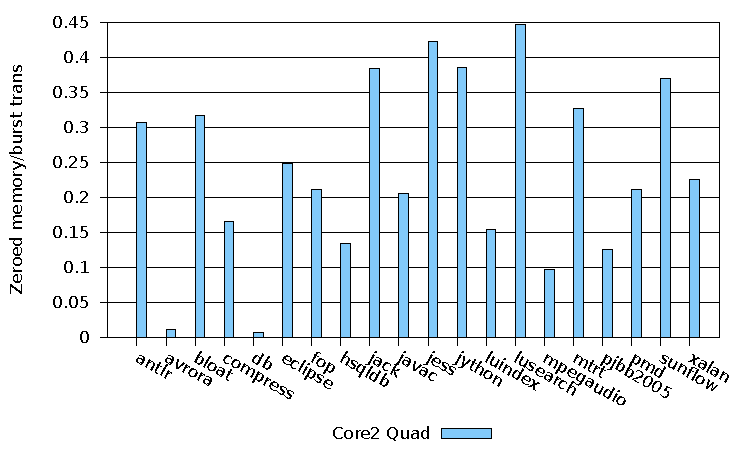
\includegraphics[width=1.0\columnwidth]{figs/zerobus_core.pdf}}



\end{figure*}


\subsection{Analysis}
%%%%%%%%%%%%
%%%%%%%%%%%%

\section{Extended Tiger}\
\label{sec:extended_tiger}
\subsection{Agent Performance} 

\begin{figure*}[!hbtp]
  \label{fig:cost}
  \makebox[\textwidth]{\framebox[5cm]{\rule{0pt}{5cm}}}
\caption{This is a placeholder.{\label{cheese_maze_performance}}}
  
 % \subfigure[Fraction of cycles spent on zeroing\label{fig:zerocost}]{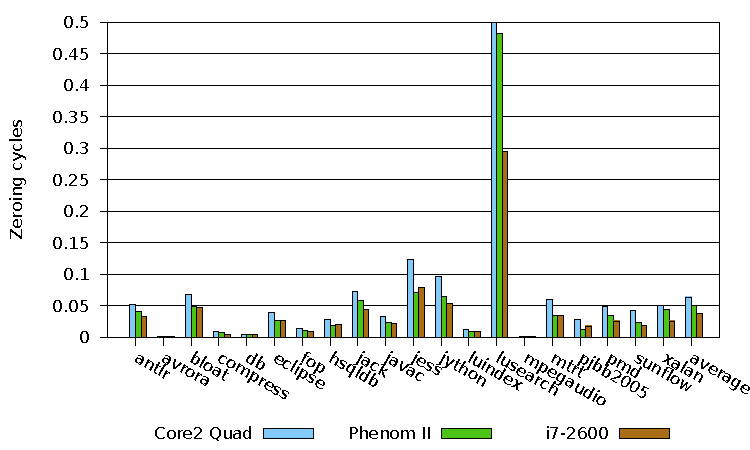
\includegraphics[width=\columnwidth]{figs/zerocost_intel.pdf}}
%  \subfigure[BytesZeroed / BytesBurstTransactionsTransferred\label{fig:zerobus}]{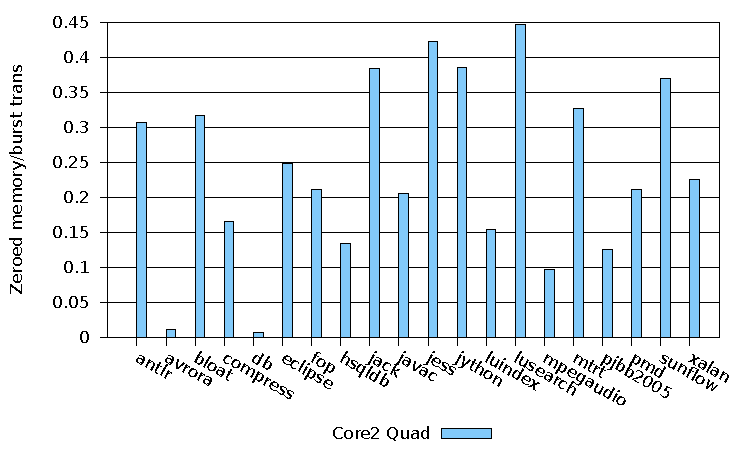
\includegraphics[width=1.0\columnwidth]{figs/zerobus_core.pdf}}



\end{figure*}



\subsection{Analysis}

%%%%%%%%%%%%
%%%%%%%%%%%%
\section{Cheese Maze}\
\label{sec:cheese_maze}
\subsection{Agent Performance} 


\begin{figure*}[!hbtp]
  \label{fig:cost}
  \makebox[\textwidth]{\framebox[5cm]{\rule{0pt}{5cm}}}
\caption{This is a placeholder.{\label{cheese_maze_performance}}}
  
 % \subfigure[Fraction of cycles spent on zeroing\label{fig:zerocost}]{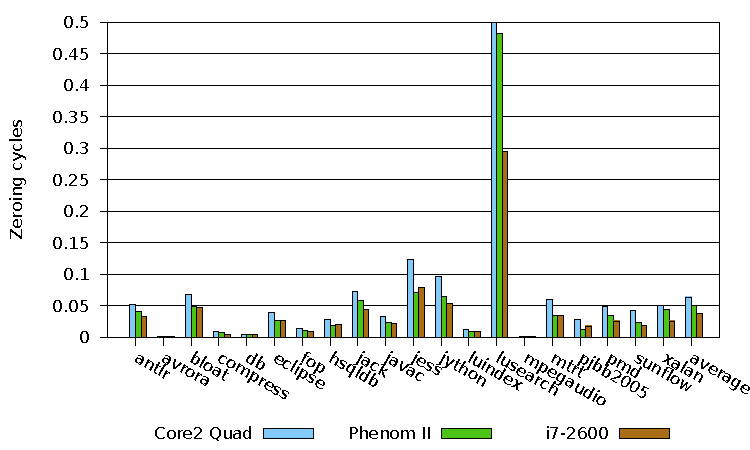
\includegraphics[width=\columnwidth]{figs/zerocost_intel.pdf}}
%  \subfigure[BytesZeroed / BytesBurstTransactionsTransferred\label{fig:zerobus}]{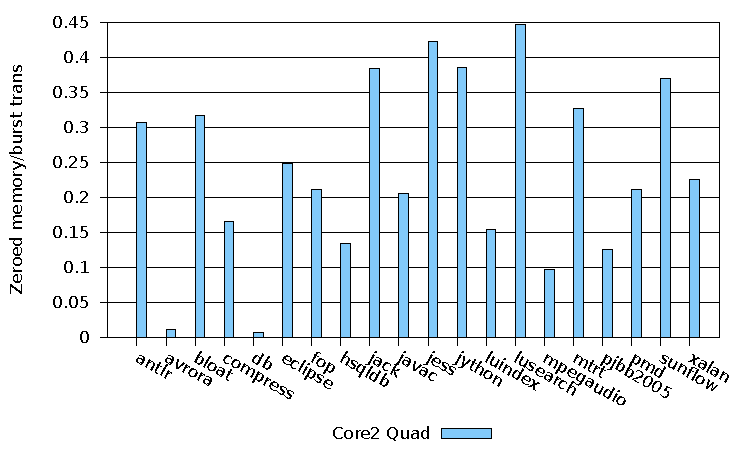
\includegraphics[width=1.0\columnwidth]{figs/zerobus_core.pdf}}



\end{figure*}


\subsection{Analysis}

%%%%%%%%%%%%
%%%%%%%%%%%%

\section{Additional Questions}\
\label{sec:cheese_maze}
\begin{enumerate}
\item
Train AIXI on d1 and then continue with d2 (without resetting the CTW and UCT). Is AIXI performing better or worse in learning d2, after having been biased towards d1, compared to training on d2 from scratch?

\item
Now go back to d1 and train AIXI on d1 again (without resetting the CTW and UCT). Does AIXI remember d1 and how fast does it recover it?
\end{enumerate}




%%%%%%%%%%%%
%%%%%%%%%%%%

Here is the example to show how to include a figure. Figure~\ref{fig:cost}
includes two subfigures (Figure~\ref{fig:zerocost}, and Figure~\ref{fig:zerobus});

\begin{figure*}
  \label{fig:cost}
  \subfigure[Fraction of cycles spent on zeroing\label{fig:zerocost}]{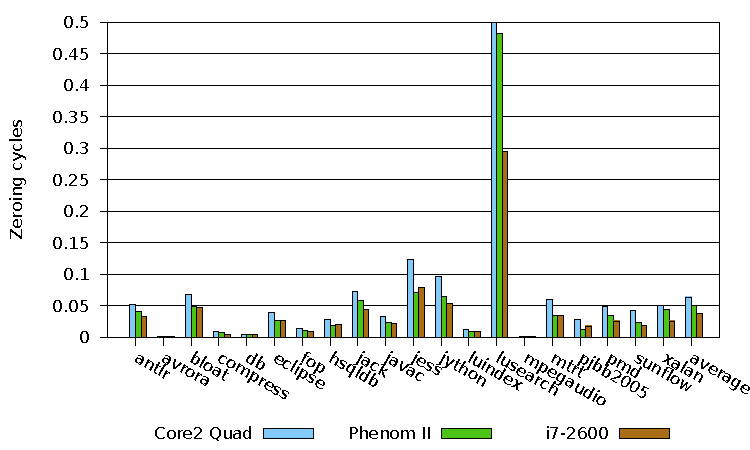
\includegraphics[width=\columnwidth]{figs/zerocost_intel.pdf}}
  \subfigure[BytesZeroed / BytesBurstTransactionsTransferred\label{fig:zerobus}]{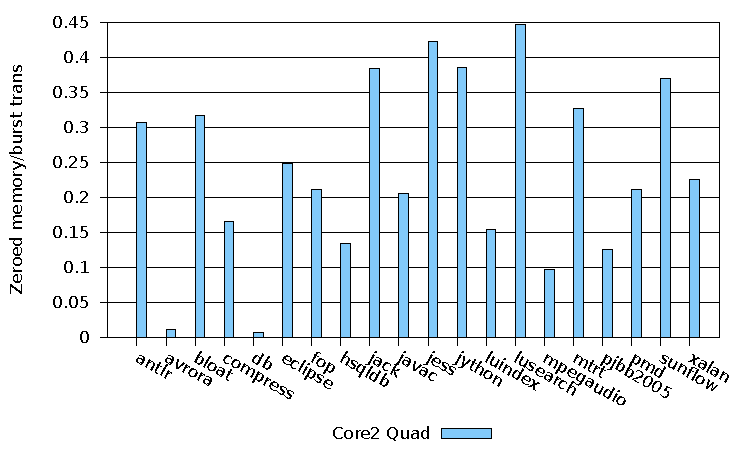
\includegraphics[width=1.0\columnwidth]{figs/zerobus_core.pdf}}
  \caption{The cost of zero initialization}
\end{figure*}


\section{Summary}
